\documentclass{optica-article}

\journal{opticajournal}
\articletype{Research Article}

\usepackage{lineno}
\usepackage[section]{placeins}
\linenumbers

\begin{document}

\title{Spectral-folding model and capacity boundary for Laguerre--Gaussian mode sorting in Fabry--P\'erot cavities}

\author{Wan-Jiang Li\authormark{1}, Deng-Hui Peng\authormark{1}, Zi-Teng Xiao\authormark{1}, Ting-Yu Yang\authormark{1}, Jian-Lan Chen\authormark{2,5}, and Han Zhang\authormark{1,3,4,6}}

\address{\authormark{1}National Laboratory of Solid State Microstructures, School of Physics, Nanjing University, Nanjing 210093, China\\
\authormark{2}School of Physics, Anhui University, Hefei 230039, China\\
\authormark{3}Hefei National Laboratory, Hefei 230088, China\\
\authormark{4}Jiangsu Key Laboratory of Quantum Information Science and Technology, Nanjing University, China}

\email{\authormark{5}cjl@ahu.edu.cn}
\email{\authormark{6}zhanghan@nju.edu.cn}

%% --- OLD abstract (commented out for reference) ---
% \begin{abstract*}
% Fabry--P\'erot (FP) cavities provide a state-preserving platform for sorting orbital angular momentum (OAM) states of light, with applications in optical communications and quantum information processing. However, a general design framework for high-dimensional LG mode sorting in FP cavities has been lacking. Here, we present an analytic design framework based on spectral folding. By mapping folded resonance positions onto a single-FSR circle, the cavity design problem is reduced to maximizing the minimum circular spacing between target modes. A unified performance criterion then relates this spacing, together with cavity finesse, to practical sorting metrics such as efficiency and extinction ratio. This framework applies to arbitrary finite target sets of LG transverse orders. For uniform-step target sets, it yields closed-form optimal cavity geometries and an analytic capacity boundary under a prescribed performance threshold. For general nonuniform target sets, it reduces the design problem to an exact finite search over bounded rational candidates. To experimentally validate the framework, we investigate a representative boundary case with nine consecutive LG modes. Measured spectra confirm the folded resonance ordering, and sorting an equal-weight 9-mode superposition yields an overall accuracy exceeding 92\%, in close agreement with the theoretical performance boundary.
% \end{abstract*}
%% --- END OLD abstract ---

%% --- NEW abstract ---
\begin{abstract*}
Fabry--P\'erot (FP) cavities provide a state-preserving platform for sorting orbital angular momentum (OAM) states of light, with applications in optical communications and photonic quantum information processing. However, a general analytical model for high-dimensional Laguerre--Gaussian (LG) mode sorting in FP cavities has been lacking. Here, we present an analytical model based on spectral folding in FP cavities. By mapping folded resonance positions onto a single free spectral range (FSR) circle, the cavity design problem is reduced to maximizing the minimum circular spacing between target modes. A unified performance criterion then links this spacing and the cavity finesse to practical sorting metrics such as sorting efficiency and extinction ratio, establishing a capacity boundary for arbitrary finite target sets under a given performance threshold. The bound is tight for uniform-step target sets, for which the optimal cavity geometry is derived in closed form; for general nonuniform sets, the design reduces to an exact finite search over a bounded set of rational candidates. To experimentally validate the model, we examine a representative boundary case involving nine consecutive LG modes. Experimental measurements confirm the predicted folded resonance ordering, where the next mode returns to the fundamental's spectral neighborhood. For an equal-weight nine-mode superposition state, the sorting achieves an average efficiency of 93.19\% and a mean extinction ratio of \(11.41\,\mathrm{dB}\) across all target modes, closely matching theoretical predictions.
\end{abstract*}
%% --- END NEW abstract ---

%% --- BEGIN merged from sections/introduction.tex ---
\section{Introduction}

%% --- PREVIOUS paragraph 1 (commented out for reference) ---
% Laguerre--Gaussian (LG) modes carrying orbital angular momentum (OAM) provide an important degree of freedom for high-dimensional photonics \cite{Allen1992,Shen2019_LSA}. They have been used in free-space and fiber optical communications, high-dimensional quantum communication, and quantum gate operations based on spatial modes \cite{Gibson2004,Wang2012_NatPhoton,Bozinovic2013,Cozzolino2019,Brandt2020,Erhard2020}. In these applications, target modes often need to be separated while retaining their original transverse field structures to support subsequent interference, routing, and further information processing tasks. Existing mode-sorting approaches include coordinate transformations, mode-conversion schemes, cascaded interferometric architectures, and, more recently, single-plane diffractive and modulo-based designs \cite{Leach2002,Berkhout2010,Mirhosseini2013,Labroille2014,Fontaine2019,Wen2018,Wen2020,Cohen2026_OE,Hu2025_NatPhoton}. These methods provide powerful mode discrimination and have achieved impressive mode capacities. A distinct class of applications---including state-preserving quantum logic gates, reconfigurable OAM routing, and modular channel switching---further requires that each sorted mode retains its original transverse field structure at the output port. Fabry--P\'erot (FP) cavities address this requirement, because they operate in the spectral domain while leaving the native transverse field intact for subsequent use.
%% --- END PREVIOUS paragraph 1 ---

%% --- PREVIOUS active introduction draft (commented out for reference) ---
% Laguerre--Gaussian (LG) modes carrying orbital angular momentum (OAM) provide an important degree of freedom for high-dimensional photonics \cite{Allen1992,Shen2019_LSA}. They have been used in free-space and fiber optical communications, high-dimensional quantum communication, and quantum gate operations \cite{Gibson2004,Wang2012_NatPhoton,Bozinovic2013,Cozzolino2019,Brandt2020,Erhard2020}. In these applications, LG modes often need to be spatially separated and directed to distinct output ports. To date, a variety of mode-sorting approaches have been developed, including coordinate transformations, mode-conversion schemes, cascaded interferometric architectures, and single-plane diffractive and modulo-based designs \cite{Leach2002,Berkhout2010,Mirhosseini2013,Labroille2014,Fontaine2019,Wen2018,Wen2020,Cohen2026_OE,Hu2025_NatPhoton}. While these methods achieve effective mode discrimination, they generally modify the transverse-field representation during sorting rather than preserving the original transverse field structure at the output port. In contrast, applications such as quantum logic gates and modular OAM processing require a state-preserving sorting stage in which each mode retains its native transverse field for subsequent processing~\cite{Brandt2020,Wei2020_Light}. Fabry--P\'erot (FP) cavities meet this requirement. By exploiting Gouy-phase-dependent resonance \cite{Kogelnik1966,Siegman1986}, an FP cavity separates modes in the spectral domain while leaving the native transverse field intact.
%
% Recent studies have demonstrated this capability in several settings. Wei et al.\ realized active sorting of low-order OAM states using cascaded tunable FP resonators \cite{Wei2020_Light}, and Vanani et al.\ extended FP-based mode selectivity to low-crosstalk mode-group demultiplexing with thin-film filters \cite{Vanani2022}. Yang et al.\ employed FP cavities as OAM-selective elements in a nonreciprocal interferometric architecture for cyclic transformations \cite{Yang2024_PRJ}. In a complementary regime, Yaraghi et al.\ demonstrated that an intra-cavity mode-converter suppresses discrete resonances via unrestricted OAM ladder-up, reshaping rather than exploiting the cavity spectral response \cite{Yaraghi2025}. While these studies establish FP cavities as a versatile platform for transverse-mode spectral engineering, a general analytical model for high-dimensional LG mode sorting in FP cavities is still lacking.
%
% For high-dimensional FP mode sorting, the key difficulty is not linewidth narrowing alone. Cavity geometry redistributes target-mode resonances within a single free spectral range (FSR), with higher-order resonances eventually folding back toward lower-order ones. As the number of target modes increases, their spectral separation becomes progressively compressed. The sorting limit is therefore set by the folded resonance arrangement together with the cavity finesse. Consequently, what is needed is a quantitative model that connects this physical picture to achievable sorting capacity and performance.
%
% In this paper, we present an analytical model based on spectral folding to address this challenge. From this model follow closed-form optimal designs for uniform-step target sets, an exact finite-search solution for general nonuniform sets, and a capacity boundary under a prescribed performance threshold. To experimentally validate the model, we investigate a representative boundary case with nine consecutive LG modes, where the next mode is predicted to return to the fundamental's spectral neighbourhood. These results provide a general basis for the design and performance prediction of high-dimensional FP mode sorters.
%% --- END PREVIOUS active introduction draft ---

LG modes carrying OAM provide a natural high-dimensional degree of freedom for photonic quantum information processing \cite{Allen1992,Shen2019_LSA}. Their high dimensionality enhances the information capacity of photonic encoding, improves noise resilience in quantum communication, and facilitates high-dimensional entanglement as well as high-dimensional gate operations \cite{Cerf2002,Cozzolino2019,Erhard2020,Brandt2020}. To harness these advantages practically, it is essential to spatially separate selected OAM modes for subsequent routing, interference, and quantum operations.

Over the past two decades, a variety of methods have been developed for sorting OAM modes. Leach et al.\ demonstrated an OAM beam splitter (OAM-BS) for odd--even sorting \cite{Leach2002}, and Slussarenko et al.\ subsequently extended this interferometric approach to a polarizing Sagnac configuration in spin--orbit photon processing \cite{Slussarenko2010}. Berkhout et al.\ proposed a log-polar coordinate transformation that maps OAM to position \cite{Berkhout2010}, and Mirhosseini et al.\ further improved its separation efficiency \cite{Mirhosseini2013}. Subsequent advances along this transformation-based approach enhanced the sorting resolution \cite{Wen2018} and enabled the modulo sorting of OAM modes \cite{Hu2025_NatPhoton}. More general approaches to spatial mode transformation have also emerged. Notably, multi-plane light conversion (MPLC) establishes a flexible platform for sorting modes across a wider range of spatial-mode bases \cite{Labroille2014} and has since been extended to the LG basis \cite{Fontaine2019}. More recently, FP-based approaches have been demonstrated for OAM-selective operations. Specifically, Wei et al.\ realized active sorting using cascaded tunable resonators \cite{Wei2020_Light}, Vanani et al.\ extended FP-based mode selectivity to low-crosstalk mode-group demultiplexing with thin-film filters \cite{Vanani2022}, and Yang et al.\ employed FP cavities as OAM-selective elements within an interferometric architecture for cyclic transformations \cite{Yang2024_PRJ}.

These developments establish multiple technical routes for OAM discrimination. But their roles in quantum information processing are not identical. In practical scenarios, once high-dimensional quantum superposition or entangled states are generated, they necessitate both mode sorting and logic gate operations. Critically, the output states following sorting should preserve their original transverse spatial mode, amplitude and phase to facilitate further operations \cite{Babazadeh2017_PRL,Brandt2020}. In this context, state preservation constitutes a core requirement for OAM sorting in the field of OAM-based optical quantum information processing.

Among existing approaches, an early state-preserving scheme is the interferometric OAM-BS. This device utilizes OAM-dependent phase shifts induced by Dove prisms in a Mach--Zehnder (M-Z) interferometer to route different OAM components to separate output ports while maintaining their original state form \cite{Leach2002,Slussarenko2010}. However, its limitation lies in its scalability to higher dimensions: accommodating an increasing number of target modes necessitates cascading additional M-Z interferometers, leading to a substantial rise in component count and imposing rigorous demands on phase stability. In contrast, FP cavities provide a different route to state-preserving OAM sorting. By exploiting Gouy-phase-dependent resonance \cite{Kogelnik1966,Siegman1986}, an FP cavity achieves spectral-domain selection of transverse modes while leaving both the transmitted and reflected fields in their original state forms. Furthermore, FP-based OAM sorting is inherently dynamically tunable and modular: the target mode can be reconfigured by varying the cavity length, and the mode count can be scaled by appending modules at the cascade output without affecting preexisting ones \cite{Wei2020_Light}. These features make FP cavities attractive for coherent routing of OAM quantum states.

Existing FP-based studies have validated the feasibility of state-preserving OAM mode-selective operations in several scenarios \cite{Wei2020_Light,Vanani2022,Yang2024_PRJ}. However, these demonstrations have largely been confined to low-order or application-specific regimes and have not yielded a general design method for a chosen target-mode set with desired sorting performance.

In this work, we develop an analytical design model for high-dimensional LG mode sorting in FP cavities. The model addresses three practical design questions: how to choose the cavity geometry for a given target-mode set, how much finesse is required to achieve a desired sorting performance, and how many modes can be supported before spectral overlap becomes the limiting factor. Built on a spectral-folding description of cavity resonances, the model yields a capacity rule, closed-form optimal solutions for uniform-step target sets, and an exact search method for general finite sets. To validate the theory, we use the model to design and fabricate an FP cavity for a nine-mode target set and experimentally test its predictions.

%% --- PREVIOUS paragraph 2 versions (commented out for reference) ---
% [v1] This state-preserving capability originates from Gouy-phase-dependent resonance in the cavity \cite{Kogelnik1966,Siegman1986}. Recent studies have demonstrated the feasibility of this mechanism in several settings. Wei et al.\ realized active sorting of low-order OAM states using cascaded tunable FP resonators \cite{Wei2020_Light}, Vanani et al.\ extended FP-based mode selectivity to low-crosstalk mode-group demultiplexing with thin-film filters \cite{Vanani2022}, and Yang et al.\ employed FP cavities as OAM-selective elements in a nonreciprocal interferometric architecture for cyclic transformations \cite{Yang2024_PRJ}. While these demonstrations establish FP cavities as a practical platform for state-preserving mode selectivity, they remain focused on specific devices or architectures. A unified analytic framework for high-dimensional LG mode sorting in FP cavities is still lacking.
% [v2] This state-preserving capability originates from Gouy-phase-dependent resonance in the cavity \cite{Kogelnik1966,Siegman1986}. Recent studies have demonstrated the feasibility of this mechanism in several settings. Wei et al.\ realized active sorting of low-order OAM states using cascaded tunable FP resonators \cite{Wei2020_Light}, Vanani et al.\ extended FP-based mode selectivity to low-crosstalk mode-group demultiplexing with thin-film filters \cite{Vanani2022}, Yang et al.\ employed FP cavities as OAM-selective elements in a nonreciprocal interferometric architecture for cyclic transformations \cite{Yang2024_PRJ}, and Yaraghi et al.\ showed that an intra-cavity mode-converter suppresses discrete resonances altogether via unrestricted OAM ladder-up, demonstrating a complementary regime in which spatial mode modification reshapes---rather than exploits---the cavity spectral response \cite{Yaraghi2025}. These studies establish FP cavities as a versatile platform for state-preserving mode selectivity and spectral engineering, yet they address specific device configurations rather than the general design question: for a given cavity finesse, how many modes can be sorted at a prescribed isolation level, and what geometry optimizes this capacity?
%% --- END PREVIOUS paragraph 2 versions ---

%% --- PREVIOUS paragraph 4 versions (commented out for reference) ---
% [v1] In this paper, we present a unified analytic design framework for high-dimensional LG mode sorting in FP cavities based on spectral folding. The framework yields closed-form optimal designs for uniform-step target sets and establishes an exact finite-search solution for general nonuniform sets. To experimentally validate this framework, we investigate a representative boundary case using nine consecutive LG modes. These results provide a general basis for the design and performance prediction of high-dimensional FP mode sorters.
% [v2] In this paper, we present an analytic design framework for LG mode sorting in FP cavities based on spectral folding. The framework maps target-mode resonances onto a single-FSR circle via modular reduction of the Gouy-phase offset and uses a spacing-based resolvability criterion to connect cavity geometry and finesse to sorting performance. From this physical model follow a universal capacity boundary applicable to arbitrary target sets, closed-form optimal geometries for uniform-step sets, and an exact finite search for general nonuniform sets. We validate the framework in the $p{=}0$ subspace at the $M{=}9$ consecutive capacity boundary, where the next mode is predicted to collide spectrally with the fundamental. Because the closed-form geometry solutions and the rational-search procedure follow deductively from the underlying physical model, a boundary-case experiment that tests the model's foundational layers provides direct support for the broader design predictions. The measured folded resonance arrangement, the spacing-determined crosstalk pattern, and the per-mode extinction ratios each test a distinct layer of this model, and all three are quantitatively consistent with the analytic predictions.
%% --- END PREVIOUS paragraph 4 versions ---
%% --- END merged from sections/introduction.tex ---
%% --- BEGIN merged from sections/design_framework.tex ---
\section{Spectral-Folding Model and Design Criterion}

In FP cavities, the resonance conditions of LG transverse modes are governed by the cavity geometry through the Gouy phase~\cite{Kogelnik1966,Siegman1986}. In a stable two-mirror configuration, each LG mode accumulates a single-pass Gouy phase shift proportional to its transverse mode order $N=2p+|l|+1$, where $p$ and $l$ are the radial and azimuthal indices, respectively. Consequently, modes with distinct values of $N$ exhibit distinct resonance frequencies within a given FSR. As the number of target modes grows, the cumulative Gouy phase shift for higher-order modes eventually exceeds one FSR, leading to a spectral wraparound effect in which the resonance frequencies of these modes revert toward the spectral positions originally occupied by lower-order modes.

\begin{figure}[htbp]
\centering
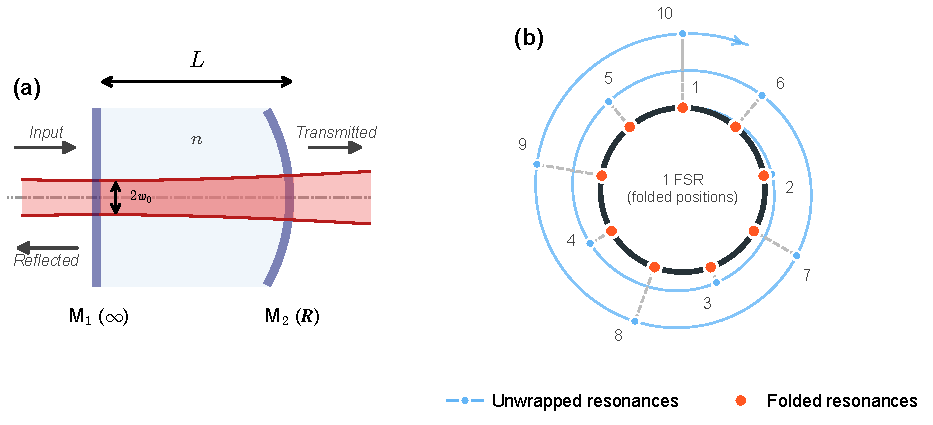
\includegraphics[width=0.92\textwidth]{figures/main/fig01_cavity_gouy_spiral}
\caption{Geometric origin of transverse-mode resonances and their single-FSR folded representation in a plane-concave cavity. (a)~A plane-concave cavity ($L$, concave radius $R$) supports LG transverse modes with Gouy-phase-dependent resonance, enabling mode-selective spectral transmission while preserving the transverse field. (b)~Archimedean-spiral representation of the single-FSR redistribution: mode $N$ lies on the outer spiral at a radius proportional to the accumulated Gouy offset $(N{-}1)k$. Its radial projection onto the inner circle (spanning one FSR) yields the folded position $\mathrm{pos}(N)=((N{-}1)k)\bmod~1$ (orange dots). For the illustrative case $k=2/9$ ($M=9$), modes $N=1$--$9$ ($l=0$--$8$) land on nine uniformly spaced folded positions; mode $N=10$ ($l=9$) wraps back to the $N=1$ neighborhood. The circular representation provides the geometric basis for defining the pairwise spacing $s_{ij}$ and the minimum spacing $s_{\min}$ used in the unified design criterion.}
\label{fig:oe_folding_concept}
\end{figure}

To develop the design criterion in the simplest explicit form, we first consider a stable plane-concave FP cavity of length $L$ and concave-mirror radius of curvature $R$, as shown in Fig.~\ref{fig:oe_folding_concept}(a). In this configuration, the resonance mode distribution within one FSR is a fixed geometric property of the cavity, governed solely by the ratio $L/R$.

To systematically analyze this periodic structure, we reduce all resonance positions modulo one FSR and map them onto a unit circle, a procedure referred to as \emph{spectral folding}. On this circle, each target mode corresponds to an angular position, and pairwise mode separations are represented as arc lengths, enabling direct comparison and optimization. Fig.~\ref{fig:oe_folding_concept}(b) illustrates this mapping: the Gouy phase offset winds outward along an Archimedean spiral, and its radial projection onto the inner circle recovers the folded positions within one FSR. Based on this circular representation, we formulate a unified analytical model applicable to arbitrary finite sets of target LG transverse orders. The extension to more general stable two-mirror cavities, including symmetric double-concave cavities, is provided in Appendix~C.

Quantitatively, for the plane-concave geometry under consideration, the resonance frequencies are given by
\begin{equation}
\nu_{q,N} = \mathrm{FSR}\!\left(q + N\frac{\phi}{\pi}\right),
\label{eq:oe_resonance}
\end{equation}
where $q$ is the longitudinal mode index, $\phi=\arccos\!\bigl(\sqrt{1-L/R}\bigr)$ is the single-pass Gouy phase, $\mathrm{FSR}=c/(2nL)$ is the free spectral range, and $n$ is the intracavity refractive index. In terms of the normalized Gouy phase shift $\phi/\pi$, which represents the transverse mode spacing relative to the FSR,
\begin{equation}
k \equiv \frac{\phi}{\pi} = \frac{1}{\pi}\arccos\!\left(\sqrt{1-\frac{L}{R}}\right),
\label{eq:oe_k_def}
\end{equation}
which depends only on the geometry ratio $L/R$, the normalized resonance position within one FSR consequently reduces to
\begin{equation}
\mathrm{pos}(N) = (Nk)\bmod~1.
\label{eq:oe_pos}
\end{equation}
The longitudinal index $q$ is eliminated by the modulo operation, so the folded arrangement depends solely on $k$. Shifting the origin to the fundamental mode yields the equivalent expression
\begin{equation}
\mathrm{pos}(N) = \bigl((N-1)k\bigr)\bmod~1.
\label{eq:oe_pos_l}
\end{equation}
This leaves all pairwise spacings invariant. Since $k$ depends only on $L/R$, the folded arrangement remains unchanged under any tuning that preserves $L/R$, whether via wavelength, refractive index, or subwavelength cavity-length scanning.

By mapping the unit interval $[0,1)$ onto a circle, each target mode is represented as a point. The design objective thereby reduces to maximizing the minimum angular separation among these points. For a target set of $M$ modes (where $M$ is the number of modes to be sorted), the relevant separation between modes $N_i$ and $N_j$ is given by the shorter arc length
\begin{equation}
s_{ij}=\min\!\left(|\mathrm{pos}(N_i)-\mathrm{pos}(N_j)|,\;1-|\mathrm{pos}(N_i)-\mathrm{pos}(N_j)|\right),
\label{eq:oe_sij}
\end{equation}
and the performance is limited by the minimum pairwise spacing
\begin{equation}
s_{\min}=\min_{i\neq j}s_{ij}.
\label{eq:oe_smin}
\end{equation}
The design task is to choose $k$ (equivalently $L/R$) so as to maximize $s_{\min}$. An elementary bound constrains this maximum: $M$ points partition the circle into $M$ arcs whose lengths sum to unity, so
\begin{equation}
s_{\min}\le \frac{1}{M},
\label{eq:oe_smin_upper}
\end{equation}
with equality if and only if the points are uniformly spaced. This geometric upper bound is universal, applying to every target set irrespective of its detailed structure. The degree to which a given set approaches this bound is determined by the algebraic properties of the order differences, as demonstrated by the two representative cases considered below.

\begin{figure}[htbp]
\centering
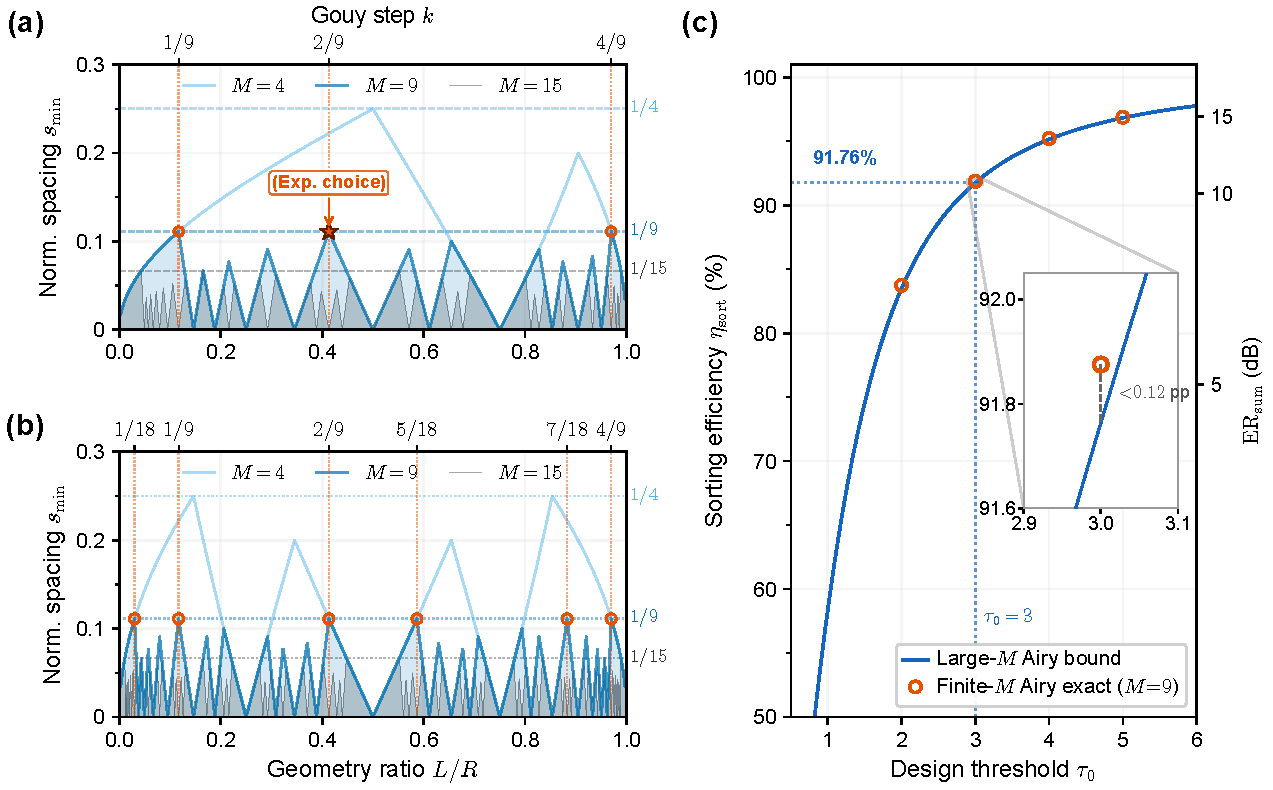
\includegraphics[width=\textwidth]{figures/main/fig02_combined}
\caption{Unified minimum-spacing criterion and its branch-specific design realizations. (a)~Representative consecutive target sets: normalized minimum spacing $s_{\min}$ versus geometry ratio $L/R$ for $M=4$, $9$, and $15$. For $M=9$ the three coprime peaks ($m=1,2,4$) each reach the ideal maximum of $1/9$; the star marks the adopted $m=2$ branch ($k^*=2/9$, $(L/R)^*\approx 0.4132$). (b)~Uniform-step target sets with $\Delta_{\mathrm{ord}}=2$: same layout as~(a) for $M=4$, $9$, and $15$. The coprime branches shift to $k=m/(2M)$ positions [Eq.~(\ref{eq:oe_uniform_condition})], but every curve still saturates its $1/M$ ceiling. For $M=9$, the number of non-redundant branches increases from three to six, including the adopted $k^*=2/9$ from the consecutive design. (c)~Conservative sorting efficiency $\eta_{\mathrm{sort}}$ and system extinction ratio $\mathrm{ER}_{\mathrm{sum}}$ versus design threshold $\tau_0$ in the large-$M$ Airy limit [Eq.~(\ref{eq:oe_pnoise_inf})]. Orange open circles are the exact finite-$M$ Airy predictions for $M=9$ at $\tau_0=2$--$5$, all within $0.5$ percentage points of the bound (see inset). The dotted crosshair marks the adopted $\tau_0=3$, corresponding to $\eta_{\mathrm{sort}}=91.76\%$ and $\mathrm{ER}_{\mathrm{sum}}>10.47\,\mathrm{dB}$.}
\label{fig:oe_design_landscape}
\end{figure}

\subsection{Representative branch: consecutive and uniform-step target sets}

For the consecutive target set $S_M=\{1,2,\dots,M\}$, the folded positions given by $\{0,k,2k,\dots,\allowbreak(M{-}1)k\}\allowbreak\bmod~1$ constitute an arithmetic progression on the circle. Consequently, uniform spacing of $1/M$ is attainable when $k$ takes the fractional value $m/M$ satisfying $\gcd(m,M)=1$, yielding
\begin{equation}
k^* = \frac{m}{M},\qquad \gcd(m,M)=1,\qquad (L/R)^* = \sin^2\!\left(\frac{\pi m}{M}\right),
\label{eq:oe_kstar}
\end{equation}
and saturating the geometric ceiling at $s_{\min}=1/M$, as depicted in Fig.~\ref{fig:oe_design_landscape}(a).

For $M=9$, the coprimality condition yields three non-redundant branches, namely $m\in\{1,2,4\}$, considering the symmetry $m\leftrightarrow M{-}m$. Each branch attains the ideal spacing $1/9$. These branches, however, exhibit different sensitivities to fabrication tolerances. The geometry-to-step derivative can be expressed as
\[
\frac{dk}{d(L/R)}=\frac{1}{2\pi\sqrt{(L/R)(1-L/R)}}.
\]
It is minimized at $L/R=0.5$. Consequently, branches for which the optimal geometry ratio $(L/R)^*$ is closer to the midpoint $L/R=0.5$ display enhanced resilience to manufacturing uncertainties in the cavity geometry. Evaluation of this derivative at the three branch points yields $dk/d(L/R)=0.495$ for $m=1$, corresponding to $(L/R)^*\approx0.117$; $0.323$ for $m=2$, corresponding to $(L/R)^*\approx0.413$; and $0.931$ for $m=4$, corresponding to $(L/R)^*\approx0.970$. Thus, for a fixed tolerance in $L/R$, the resulting shifts in $k$ are $1.5\times$ and $2.9\times$ larger for the $m=1$ and $m=4$ branches, respectively, relative to the observed minimum at $m=2$. The $m=2$ branch is adopted for the experiment reported below, for its combination of optimal spacing and the lowest sensitivity among the three branches.

The consecutive case represents the simplest instance of a more general uniform-step family. When the target mode indices follow an arithmetic progression $N_i=N_0+(i-1)\Delta_{\mathrm{ord}}$, a change in the starting index $N_0$ merely results in a global rotation of the points on the circle. The step size $\Delta_{\mathrm{ord}}$, in contrast, defines an effective circular increment,
\begin{equation}
u=(\Delta_{\mathrm{ord}}\,k)\bmod~1.
\label{eq:oe_u_def}
\end{equation}
In terms of $u$, a uniform-step set of $M$ modes is equivalent to an $M$-mode consecutive problem. The geometric ceiling $s_{\min}=1/M$ is therefore attained when the following coprimality condition is satisfied:
\begin{equation}
\Delta_{\mathrm{ord}}\,k \equiv \frac{m}{M}\pmod{1},\qquad \gcd(m,M)=1.
\label{eq:oe_uniform_condition}
\end{equation}
The corresponding cavity geometry is given by $L/R=\sin^2(\pi k)$. The entire uniform-step family thus saturates the $1/M$ bound. This is illustrated in Fig.~\ref{fig:oe_design_landscape}(b) for $\Delta_{\mathrm{ord}}=2$: for $M=9$, the landscape now admits six coprime branches reaching $s_{\min}=1/9$, compared with only three in the consecutive case, while $M=4$ and $M=15$ retain their respective ceilings. The adopted geometry $k^*=2/9$ remains optimal for both step sizes.

\subsection{Extension to general target sets}

The model is not restricted to uniform-step progressions. For a general target set $S=\{N_1,\dots,\allowbreak N_M\}$\allowbreak\ with pairwise order differences $D(S)=\{N_j-N_i:\allowbreak i<j\}$, the minimum spacing takes the form
\begin{equation}
s_{\min}(k;S) = \min_{d\in D(S)} \|d\,k\|,
\label{eq:oe_smin_general}
\end{equation}
where $\|x\|$ denotes the distance from $x$ to its nearest integer. Over any rational search window $I=[a,b]$, this function is the piecewise-linear lower envelope of finitely many V-shaped profiles $\|d\,k-n\|$, so its global maximum is attained at a rational value $k^*=m/q$ whose denominator satisfies an explicit bound
\begin{equation}
q \le Q_I(S) = \max\!\bigl(\mathrm{den}(a),\,\mathrm{den}(b),\,2D_{\max}\bigr),\qquad D_{\max}=\max D(S).
\label{eq:oe_Q_bound}
\end{equation}
where $\mathrm{den}(\cdot)$ denotes the denominator of a rational number written in lowest terms.
The design problem therefore reduces to an exact search over finitely many rational candidates $(m,q)$ with $\gcd(m,q)=1$ and $a\le m/q\le b$. For uniform-step sets, this recovers the closed-form result of the preceding subsection; for general finite sets, it provides the corresponding optimum without a continuous scan. A proof is provided in Appendix A.2.

\subsection{Resolvability criterion and unified capacity boundary}

So far the analysis has established how to maximize the minimum spacing $s_{\min}$ for a given target set. To translate this geometric spacing into a physical crosstalk level, it must be compared with the spectral width of the cavity transmission peak.

Each resonance of the FP cavity has a full width at half maximum $\mathrm{FWHM}=\mathrm{FSR}/\mathcal{F}$, where $\mathcal{F}$ is the cavity finesse. The physical frequency gap between two modes with circular spacing $s_{ij}$ is $\Delta\nu_{ij}=s_{ij}\cdot\mathrm{FSR}$. Dividing this frequency gap by the linewidth yields their separation in units of linewidths:
\begin{equation}
\tau_{ij}\equiv \frac{\Delta\nu_{ij}}{\mathrm{FWHM}}
=\mathcal{F}\cdot s_{ij},
\qquad
\tau_{\min}=\mathcal{F}\cdot s_{\min}.
\label{eq:oe_tau}
\end{equation}
$\tau$ counts how many linewidths separate two peaks. The pair with the smallest $\tau$ exhibits the highest crosstalk, and this bottleneck value is denoted $\tau_{\min}$.
To impose a design requirement on mode isolation, we introduce a threshold $\tau_0$, defined as the minimum acceptable separation between any two resonances in units of linewidths.
The crosstalk at a given $\tau$ is governed by the cavity transmission lineshape. The ideal FP transmittance follows the Airy function,
\begin{equation}
T(\nu)=\frac{1}{1+\left(\dfrac{2\mathcal{F}}{\pi}\right)^{\!2}
\sin^2\!\!\left(\dfrac{\pi\nu}{\mathrm{FSR}}\right)}.
\label{eq:oe_airy}
\end{equation}
When the cavity is locked to a target mode, any non-target mode detuned by $\Delta\nu$ still transmits a fraction $T(\Delta\nu)$. This residual transmission constitutes the physical origin of inter-mode crosstalk.

For $M$ uniformly spaced target modes operating at the capacity-boundary finesse $\mathcal{F}=M\tau_0$, the total crosstalk associated with any target mode is the exact Airy circular sum
\begin{equation}
P_{\mathrm{noise}}^{(M)}(\tau_0)
=\sum_{n=1}^{M-1}
\frac{1}{1+\left(\dfrac{2M\tau_0}{\pi}\right)^{\!2}
\sin^2\!\left(\dfrac{\pi n}{M}\right)}.
\label{eq:oe_pnoise_M}
\end{equation}
This sum admits a closed-form expression (see Appendix A.1) and is a monotonically increasing function of $M$. In the asymptotic limit $M\to\infty$ with $\tau_0$ held fixed, it converges to
\begin{equation}
P_{\mathrm{noise}}^{(\infty)}(\tau_0)
=\frac{\pi}{2\tau_0}\coth\!\frac{\pi}{2\tau_0}-1,
\label{eq:oe_pnoise_inf}
\end{equation}
which is independent of $M$ and serves as a conservative upper bound on the crosstalk: for any finite $M$, $P_{\mathrm{noise}}^{(M)}<P_{\mathrm{noise}}^{(\infty)}$. The corresponding sorting efficiency and extinction ratio are given by
\begin{equation}
\mathrm{ER}_{\mathrm{sum}}^{(\infty)}=10\lg\frac{1}{P_{\mathrm{noise}}^{(\infty)}},
\qquad
\eta_{\mathrm{sort}}^{(\infty)}=\frac{1}{1+P_{\mathrm{noise}}^{(\infty)}}.
\label{eq:oe_er_eta}
\end{equation}
Taking $M=9$ at $\mathcal{F}=27$ as an example, the exact finite-$M$ prediction gives an extinction ratio of $\mathrm{ER}_{\mathrm{sum}}^{(9)}=10.53\,\mathrm{dB}$, a mere $0.06\,\mathrm{dB}$ above the conservative bound [see Fig.~\ref{fig:oe_design_landscape}(c)].

The design threshold $\tau_0$ specifies the minimum acceptable spacing between any two cavity resonances in units of linewidths. By imposing $\tau_{\min}\ge\tau_0$, the geometric frequency separation directly translates into a guaranteed isolation level. The relationship between $\tau_0$ and the corresponding conservative performance bounds is shown in Fig.~\ref{fig:oe_design_landscape}(c); numerical values for several representative thresholds are summarized in Table~\ref{tab:oe_tau_bounds}. For the threshold $\tau_0=3$ adopted throughout this work, we obtain $\eta_{\mathrm{sort}}^{(\infty)}=91.76\%$ and $\mathrm{ER}_{\mathrm{sum}}^{(\infty)}>10.47\,\mathrm{dB}$.

\begin{table}[htbp]
\centering
\caption{Conservative lower bounds on sorting performance.}
\label{tab:oe_tau_bounds}
\begin{tabular}{ccc}
\hline
$\tau_0$ & $\mathrm{ER}_{\mathrm{sum}}^{(\infty)}$ (dB) & $\eta_{\mathrm{sort}}^{(\infty)}$ (\%) \\
\hline
1.0 &  1.47 & 58.39 \\
2.0 &  7.04 & 83.50 \\
3.0 & 10.47 & 91.76 \\
4.0 & 12.93 & 95.16 \\
5.0 & 14.86 & 96.84 \\
6.0 & 16.43 & 97.78 \\
\hline
\end{tabular}

\smallskip
\begin{minipage}{4.25in}
\footnotesize
\setlength{\parindent}{0pt}
Values are the asymptotic extinction ratio $\mathrm{ER}_{\mathrm{sum}}^{(\infty)}$ and sorting efficiency $\eta_{\mathrm{sort}}^{(\infty)}$ for representative design thresholds~$\tau_0$, evaluated from the large-$M$ limit of the exact Airy circular sum. Closed-form expressions are given in Eqs.~(\ref{eq:oe_pnoise_inf}--\ref{eq:oe_er_eta}).
\end{minipage}
\end{table}

Combining the threshold condition $\tau_{\min}\ge\tau_0$ with the universal geometric upper bound $s_{\min}\le 1/M$ leads directly to the central design inequality:
\begin{equation}
M \le \left\lfloor \frac{\mathcal{F}}{\tau_0}\right\rfloor.
\label{eq:oe_capacity}
\end{equation}
This bound applies universally to any target set and any cavity geometry: a single FP cavity of finesse $\mathcal{F}$ can sort at most $\lfloor\mathcal{F}/\tau_0\rfloor$ modes at the required isolation level. For uniform-step target sets, the optimal arrangement attains the bound with $s_{\min}=1/M$. For nonuniform target sets, equality in this bound is not guaranteed: it depends on whether the set can be mapped by an admissible cavity step to an equally spaced circular arrangement. When this condition is not met, the optimum has $s_{\min}^*<1/M$, and a higher finesse is required to compensate for the resulting spacing deficit. While the analysis uses a plane-concave cavity, the model depends on~$k$. For a general stable two-mirror cavity, the step generalizes to $k_{\mathrm{eff}}=\pi^{-1}\arccos\!\bigl(\sqrt{g_1 g_2}\bigr)$ with $g_{1,2}=1-L/R_{1,2}$; all results carry over (see Appendix C).
%% --- END merged from sections/design_framework.tex ---
%% --- BEGIN merged from sections/experimental_validation.tex ---
\section{Nine-Mode Boundary-Probing Validation}

This section experimentally validates the proposed model on a representative consecutive-mode boundary. The target set consists of $M=9$ consecutive LG modes with $p=0$ ($l=0$--$8$). For this set, the closed-form optimum [Eq.~(\ref{eq:oe_kstar})] yields $k^*=2/9$ and $(L/R)^*\approx 0.4132$. In this subspace, $N=|l|+1$ gives a one-to-one correspondence between the mode label and the transverse order. The folded ordering and the first return beyond the target set can therefore be read directly from measured spectra. At this operating point, the nine target resonances are equally spaced around the single-FSR circle with a uniform spacing of $1/9$ of one $\mathrm{FSR}$, whereas the next-order mode with $l=9$ (i.e., $N=10$) returns to the neighborhood of the fundamental. This return signifies the predicted onset of spectral overlap at the nine-mode capacity boundary. For the design threshold $\tau_0=3$, the capacity inequality [Eq.~(\ref{eq:oe_capacity})] imposes a minimum finesse requirement of $\mathcal{F}_{\min}=M\tau_0=27$.

The measurement campaign establishes three key aspects of the model: (i)~the folded resonance arrangement from the single-FSR circular representation; (ii)~the crosstalk structure governed by the minimum folded spacing $s_{\min}$; (iii)~the quantitative performance bounds set by the $\tau$ criterion. In the subsequent subsections, we first demonstrate that the fabricated cavity operates at the intended design point, followed by a verification of the folded spectral arrangement and the next-mode return. We conclude with an assessment of the sorting performance under an equal-weight superposition of the nine modes as input.

\subsection{Experimental setup}
The optical layout is shown in Fig.~\ref{fig:oe_setup}. A narrow-linewidth tunable laser centered at $795\,\mathrm{nm}$ passes through a $(2.5\times)$ beam expander. The expanded beam is then addressed by a reflective phase-only spatial light modulator (SLM1), which imprints the required complex amplitude via holography~\cite{Bolduc2013} to produce the nine target $\mathrm{LG}_0^l$ modes ($l=0$--$8$). Two successive $4f$ relays perform three functions: selecting the first-order diffraction, providing spatial filtering, and matching the beam waist to the cavity mode. The prepared beam is then coupled into a temperature-stabilized fused-silica plane-concave FP cavity. The geometry ratio of this cavity is set near $(L/R)^*\approx0.4132$.

Two measurement configurations share the same input path. For spectral characterization, the laser frequency is swept over ${\approx}14.2\,\mathrm{GHz}$, and the cavity transmission is recorded by a photodetector. For the equal-weight nine-mode superposition measurement, the second spatial light modulator (SLM2) imprints conjugate holograms onto the transmitted field. The shaped field is then coupled into a single-mode fiber via a $4f$ relay lens system.

\begin{figure}[htbp]
\centering
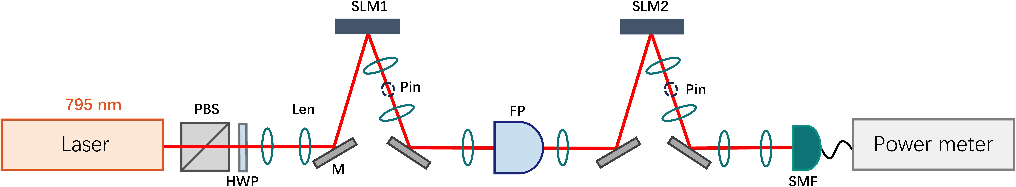
\includegraphics[width=0.88\textwidth]{figures/main/fig03_experimental_setup.pdf}
\caption{Experimental setup for the nine-mode FP-cavity sorter. A tunable laser ($795\,\mathrm{nm}$) is beam-expanded ($2.5\times$) and encoded onto a reflective phase-only SLM1 via complex-amplitude holography to generate the target $\mathrm{LG}_0^l$ modes ($l=0$--$8$). Relay optics provide first-order selection, spatial filtering, and cavity-mode matching into a temperature-stabilized plane-concave FP cavity. The schematic shows the common input path and the mode-resolved projection arm. For mode-resolved measurements with an equal-weight superposition input, the transmitted field is projected by SLM2, relayed to a single-mode fiber, and recorded by a power meter. For spectral characterization, the cavity transmission is recorded by a photodetector at the transmission port.}
\label{fig:oe_setup}
\end{figure}

\subsection{Operating-point calibration}
Frequency-domain transmission measurements confirm that the fabricated cavity operates close to the predicted design point. The measured $\mathrm{FSR}$ and finesse are $9.915\pm0.004\,\mathrm{GHz}$ and $\mathcal{F}=32.21\pm0.19$, respectively. A fit to the resonance positions yields a normalized Gouy step of $k=0.2228\pm0.0003$, within $0.3\%$ of the design value $k^*=2/9\approx0.2222$. Using the plane-concave relation between $k$ and $L/R$, this fitted step corresponds to an effective geometry ratio $(L/R)_{\mathrm{eff}}\approx0.4146$, close to the target value $(L/R)^*\approx0.4132$.

Using the nine measured target resonances, the minimum folded pairwise spacing is $s_{\min}^{\mathrm{meas}}\approx0.1086$. The corresponding linewidth-scaled resolvability is $\tau_{\min}^{\mathrm{meas}}=\mathcal{F}\,s_{\min}^{\mathrm{meas}}\approx3.50$ [Eq.~(\ref{eq:oe_tau})], placing the device above the design threshold $\tau_0=3$. At the threshold finesse $\mathcal{F}_{\min}=27$, satisfying this condition would require the nine-mode spacing to attain the geometric upper bound $s_{\min}=1/9$, leaving no spacing margin against deviations of $k$ from an exact optimal branch. The measured finesse exceeds this threshold by ${\sim}19\%$. This excess finesse provides a tolerance window of $|\Delta k|\lesssim4\times10^{-3}$ around the selected design point, as quantified in Appendix B.2.

\subsection{Spectral verification and next-mode return}
\begin{figure}[!htbp]
\centering
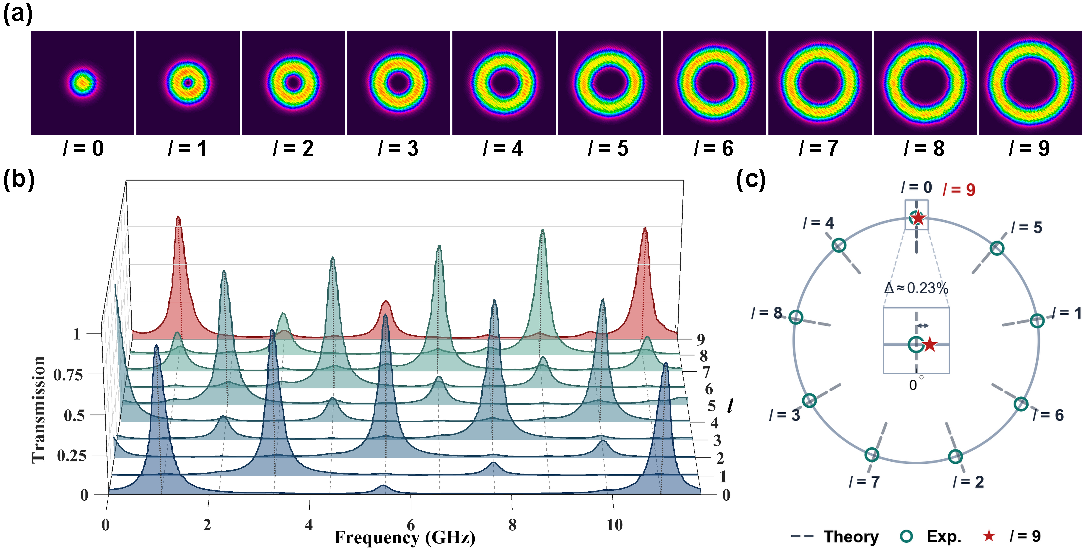
\includegraphics[width=0.95\textwidth]{figures/main/fig04_combined}
\caption{Experimental validation of the representative consecutive-mode boundary case.
(a)~Charge-coupled device (CCD) images of cavity-transmitted individual OAM modes at their respective resonance peaks ($l=0$--$9$), confirming transverse-profile preservation through the FP cavity.
(b)~Measured transmission spectra of $l=0$--$9$ within one FSR, showing the non-monotonic peak arrangement predicted by the folding model at the consecutive optimum. The $l=9$ resonance (red) returns to the $l=0$ neighborhood at the FSR boundary. Weak satellite resonances in several higher-$l$ traces are consistent with residual $p=1$ radial-mode excitation.
(c)~Polar representation of measured peak positions (circles) versus theoretical predictions (dashed, $k^*=2/9$). Inset: magnified next-mode return region showing a residual separation of $0.23\%\,\mathrm{FSR}$.}
\label{fig:oe_peak_validation}
\end{figure}

The cavity-transmitted images recorded at the resonance peaks [see Fig.~\ref{fig:oe_peak_validation}(a)] retain the expected OAM-dependent transverse structures of the target modes, confirming that the FP cavity preserves the transverse mode profile during sorting. The measured individual-mode transmission spectra [as shown in Fig.~\ref{fig:oe_peak_validation}(b)] provide a direct test of the folding prediction: within one FSR, the nine target resonances do not follow the monotonic order of the mode index but instead appear at the positions prescribed by $\mathrm{pos}(N)=((N{-}1)k)\bmod 1$ [Eq.~(\ref{eq:oe_pos_l})]. The average frequency deviation between measured and predicted peak positions is ${\approx}28\,\mathrm{MHz}$, less than one-tenth of the measured linewidth (${\approx}307\,\mathrm{MHz}$). The polar comparison in Fig.~\ref{fig:oe_peak_validation}(c) confirms this quantitative agreement across all nine target modes.

Weak satellite resonances visible in several higher-$l$ traces are consistent with residual $p=1$ radial-mode excitation from imperfect cavity-mode matching. For fixed $l$, this component is shifted by two transverse-order units relative to the intended $p=0$ mode, as follows from the mode index relation $N=2p+|l|+1$.

The folding model also predicts the spectral position of the first mode outside the target set. For $l=9$ ($N=10$), the folding formula gives $\mathrm{pos}(10)=((10{-}1)\times 2/9)\bmod 1=0$, placing this mode at the same folded position as the fundamental. The measured $l=9$ resonance [red curve in Fig.~\ref{fig:oe_peak_validation}(b); red star in Fig.~\ref{fig:oe_peak_validation}(c)] falls only $23\,\mathrm{MHz}$ (${\approx}0.07$ linewidths, $0.23\%\,\mathrm{FSR}$) from the $l=0$ resonance, confirming this predicted return at the nine-mode capacity boundary.

\subsection{Sorting performance under simultaneous nine-mode input}
\begin{figure}[htbp]
\centering
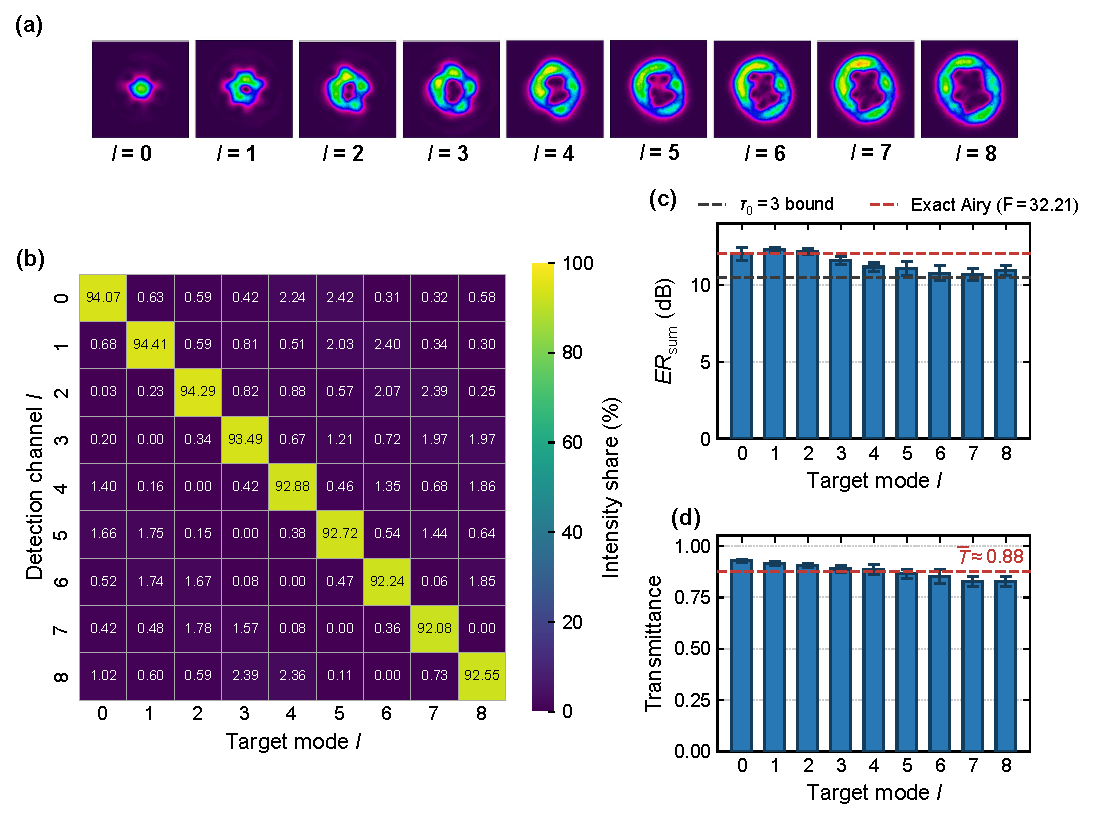
\includegraphics[width=0.95\textwidth]{figures/main/fig05_combined}
\caption{Sorting under simultaneous nine-mode input.
(a)~CCD spot patterns recorded at the $l=0$--$8$ resonance peaks.
(b)~Measured $9\times9$ normalized mode-sorting matrix with an equal-weight superposition input; diagonal entries indicate sorting efficiencies exceeding $92\%$.
(c)~Per-mode system extinction ratio ($\mathrm{ER}_{\mathrm{sum}}$) compared with the conservative large-$M$ lower bound ($10.47\,\mathrm{dB}$) and the exact finite-$M$ Airy prediction ($12.04\,\mathrm{dB}$).
(d)~Single-mode peak transmittance for $l=0$--$8$. The gradual decrease with increasing $l$ contributes to the lower extinction ratios of the higher-$l$ modes in~(c).}
\label{fig:oe_nine_mode_sorting}
\end{figure}

To evaluate the FP-cavity sorting performance in the nine-mode $\mathrm{LG}_0^l$ target basis, we injected an equal-weight superposition of all nine target modes into the cavity and read out the transmitted field by sequential projection using the projection arm consisting of SLM2 and a single-mode fiber. This projection arm readout uses conjugate complex-amplitude holograms~\cite{Bolduc2013} followed by single-mode-fiber coupling, which can introduce mode-dependent readout efficiencies and finite projection crosstalk. We independently characterized the projection arm using single-mode inputs. We obtained a readout-response matrix and used this matrix to account for the readout response in the raw projection vectors before column-wise normalization~\cite{Carpenter2014,Rehacek2010}. The resulting normalized mode-sorting matrix [see Fig.~\ref{fig:oe_nine_mode_sorting}(b)] is strongly diagonally dominant, with sorting efficiencies ranging from $92.08\%$ to $94.41\%$ and a mean sorting efficiency of $93.19\%\pm0.37\%$ (95\% confidence interval from three independent runs). Residual off-diagonal leakage is concentrated among nearest-neighbor mode pairs on the folded circle, consistent with the minimum-spacing bottleneck predicted by the model. Further details of the response-matrix procedure are provided in Appendix B.1.

The mode-resolved extinction ratios [Fig.~\ref{fig:oe_nine_mode_sorting}(c)] provide the most direct quantitative comparison with the model predictions. The model establishes two reference levels: a conservative lower bound of $10.47\,\mathrm{dB}$ set by the design threshold $\tau_0=3$ in the large-$M$ limit (Table~\ref{tab:oe_tau_bounds}), and an exact finite-$M$ Airy prediction of $12.04\,\mathrm{dB}$ evaluated at the measured finesse under equal spacing. The measured mean extinction ratio is $11.41\pm0.25\,\mathrm{dB}$, and the worst-performing mode ($l=7$) is $10.66\,\mathrm{dB}$. All modes fall above the conservative lower bound and below the ideal Airy reference level, placing the measured performance within the design regime predicted by the model. The single-mode peak transmittance in Fig.~\ref{fig:oe_nine_mode_sorting}(d) decreases gradually with increasing azimuthal index, with a mean value of $\bar{T}\approx0.88$. This trend is consistent with the larger spatial extent of higher-$l$ modes, which increases their sensitivity to finite aperture, cavity-mode matching, and input-alignment errors. It also helps explain the per-mode variation in Fig.~\ref{fig:oe_nine_mode_sorting}(c): for higher-$l$ target modes, the transmitted signal is weaker, whereas leakage from folded lower-$l$ neighbors on the folded circle can have higher peak transmittance.

Together, the operating-point calibration, the folded resonance arrangement, the next-mode return at $l=9$, and the nine-mode sorting performance complete the three-part experimental validation outlined at the beginning of this section. Design extensions and the broader applicability of the model are discussed in the following section.
%% --- END merged from sections/experimental_validation.tex ---
%% --- BEGIN merged from sections/discussion.tex ---
\section{Discussion}

The preceding experiment validates the model at the nine-mode capacity boundary. The same capacity equation sets the design scale for other mode counts: $\mathcal{F}_{\min}=M\tau_0$ increases linearly with $M$, so each additional target mode requires only $\tau_0$ units of additional finesse. Table~\ref{tab:oe_design_blueprint} lists the resulting design blueprint from $M=4$ to $M=100$ at $\tau_0=3$, including the preferred geometry branch, the corresponding $L/R$, and the predicted performance for each case. The predicted efficiency converges rapidly to the large-$M$ limit, whereas the extinction ratio varies only weakly across the table.

\begin{table}[htbp]
\centering
\caption{Consecutive-set sorting design blueprint for $\tau_0=3$.}
\label{tab:oe_design_blueprint}
\begin{tabular}{ccccccc}
\hline
$M$ & $\mathcal{F}_{\min}$ & $m$ & $k^*$ & $(L/R)^*$ & $\mathrm{ER}_{\mathrm{sum}}^{(M)}$ (dB) & $\eta_{\mathrm{sort}}^{(M)}$ (\%) \\
\hline
4 & 12 & 1 & $1/4$ & 0.5000 & 10.80 & 92.3 \\
9 & 27 & 2 & $2/9$ & 0.4132 & 10.53 & 91.9 \\
15 & 45 & 4 & $4/15$ & 0.5523 & 10.49 & 91.8 \\
30 & 90 & 7 & $7/30$ & 0.4477 & 10.48 & 91.8 \\
50 & 150 & 13 & $13/50$ & 0.5314 & 10.47 & 91.8 \\
100 & 300 & 23 & $23/100$ & 0.4373 & 10.47 & 91.8 \\
\hline
\end{tabular}

\smallskip
\begin{minipage}{4.25in}
\footnotesize
\setlength{\parindent}{0pt}
Here $\mathcal{F}_{\min}=3M$; the preferred $m$ is the coprime branch nearest the lowest-sensitivity geometry. $\mathrm{ER}$ and $\eta$ are finite-$M$ Airy predictions at $\mathcal{F}=\mathcal{F}_{\min}$; formulas are given in Appendix~A.1.
\end{minipage}
\end{table}

The present validation uses the $p{=}0$ subspace, where the transverse order $N=|l|+1$ gives a one-to-one correspondence between the mode label and~$N$ and makes the folding sequence directly observable. The design model is written for the general transverse order $N=2p+|l|+1$, and FP-based mode selectivity involving multiple radial orders has been demonstrated in related configurations~\cite{Vanani2022}. The same spacing criterion also determines the design of other finite target sets: for uniform-step target sets, equality in the capacity bound is attainable [Eq.~(\ref{eq:oe_uniform_condition})], whereas for general nonuniform sets, the best geometry follows from the exact rational search of Section~2. Since the analysis depends only on the normalized Gouy step~$k$, it is not tied to the plane-concave cavity used in the experiment. The folding analysis, crosstalk sums, and capacity bound carry over to general stable two-mirror cavities via the effective Gouy step defined in Appendix~C. Different cavity types, such as symmetric double-concave cavities, modify only the geometry-to-step mapping and the branch-sensitivity ranking; the capacity condition itself remains unchanged.

At the cavity-design level, the relevant parameters are the normalized Gouy step $k$ and the finesse $\mathcal{F}$. Because the sorting mechanism is a passive linear spectral response of the cavity, the same transfer function applies to single-photon inputs, provided the photon bandwidth remains narrow relative to the cavity linewidth. Related work has demonstrated Gouy-phase-controlled evolution in multi-photon quantum states~\cite{Hiekkamaki2022}. The capacity boundary and design rules derived here therefore provide quantitative guidance for extending FP-based mode sorting toward high-dimensional quantum information processing~\cite{Brandt2020,Cozzolino2019}.

This dimensionless structure also clarifies how the design scales. Within the model, preserving the effective Gouy step and the finesse preserves the normalized sorting performance, independent of the absolute cavity size. This property enables compact and integrated implementations. Integrated lithium-niobate FP micro-resonators, for instance, provide a compact FP platform with electro-optic intracavity refractive-index control for resonance tuning~\cite{Hwang2026_npjNano}. The present model specifies the effective Gouy step and finesse required for a target sorting capacity, thereby providing design guidance for such miniaturized FP platforms.

\section{Conclusion}

This work establishes an analytical model based on spectral folding for high-dimensional LG mode sorting in FP cavities. The single-FSR circular representation reduces cavity design to a one-parameter optimization on the normalized Gouy step~$k$. Together with the finesse, the minimum folded spacing defines the resolvability criterion $\tau_{\min}=\mathcal{F}\,s_{\min}\ge\tau_0$, which translates geometric spacing into a guaranteed isolation level and yields the capacity boundary $M\le\lfloor\mathcal{F}/\tau_0\rfloor$ for arbitrary finite target sets. A nine-mode boundary experiment quantitatively validates the model: measured resonance positions agree with predictions to within $0.1$~linewidth, the next mode returns to the fundamental's spectral neighborhood at the predicted capacity boundary, and sorting under an equal-weight superposition of all nine modes yields a mean efficiency of $93.19\%$ and a mean extinction ratio of $11.41\,\mathrm{dB}$, with all target modes falling within the predicted design regime. Because the cavity response is governed by the normalized Gouy step and the finesse, the model extends to stable two-mirror cavities through the effective Gouy step and provides a quantitative analytical basis for the design and performance prediction of high-dimensional FP mode sorters.
%% --- END merged from sections/discussion.tex ---

\begin{backmatter}
\bmsection{Funding}
This work was supported by the National Natural Science Foundation of China (Grant No. U25A6008) and the Quantum Science and Technology-National Science and Technology Major Project (Grant No. 2021ZD0301400).

\bmsection{Acknowledgment}
The authors thank Prof. Xi-lin Wang for technical support with the experiment.

\bmsection{Disclosures}
The authors declare that there are no conflicts of interest related to this article.

\bmsection{Data availability}
Data underlying the results presented in this paper are not publicly available at this time but may be obtained from the authors upon reasonable request.

\bmsection{Supplemental document}
See Supplement 1 for supporting content.
\end{backmatter}

\bibliography{bib/refs_local}

\end{document}
